In Chapter~\ref{ch:source-coding}, we saw how to encode a source such that it can be stored or sent over some channel, and decoded at a later point in time. We assumed that the channel used to send the encoded information was perfect, meaning that no information got altered or lost while being sent over the channel. In this chapter, we consider a different setting, where the channel possibly contains some \term{noise}, that may convert the channel input $x$ to some potentually different value $y$:

\begin{figure}[h]
\begin{center}
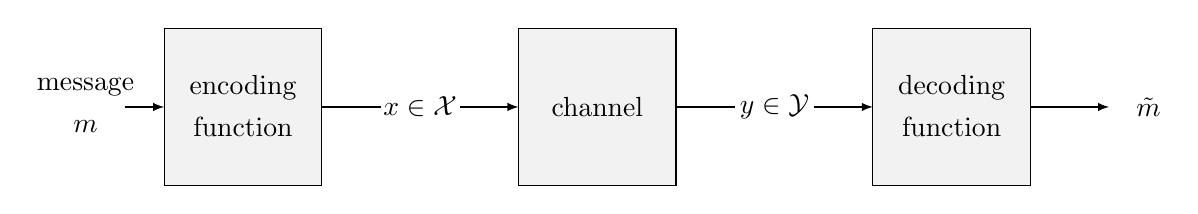
\begin{tikzpicture}
%\draw[fill=black!5] (0,0) rectangle (2,2);
%\node at (1,1.25) {$P_X$};
%\node at (1,0.75) {(source)};


%\draw[-latex] (2,1) -- (5,1);
%\draw[fill=white,draw=none] (2.5,0) rectangle (4.5,2);
%\node at (3.5,1.5) {$x$, with};
%\node at (3.5,1) {probability};
%\node at (3.5,0.5) {$P_X(x)$};
\node at (0,1.25) {message};
\node at (0,0.75) {$m$};
\draw[-latex] (0.5,1) -- (1,1);

\draw[fill=black!5] (1,0) rectangle (3,2);
\node at (2,1.25) {encoding};
\node at (2,0.75) {function};

\draw[-latex] (3,1) -- (5.5,1);
\fill[white] (3.75,0) rectangle (4.75,2);
\node at (4.25,1) {$x \in \mathcal{X}$};

\draw[fill=black!5] (5.5,0) rectangle (7.5,2);
\node at (6.5,1) {channel};

\draw[-latex] (7.5,1) -- (10,1);
\draw[fill=white,draw=none] (8.25,0) rectangle (9.25,2);
\node at (8.75,1) {$y \in \mathcal{Y}$};

\draw[fill=black!5] (10,0) rectangle (12,2);
\node at (11,1.25) {decoding};
\node at (11,0.75) {function};

\draw[-latex] (12,1) -- (13,1);
\node at (13.5,1) {$\tilde{m}$};
\end{tikzpicture}
\end{center}
\end{figure}
The goal is to design encoding and decoding functions that can resist this noise, so that the recovered message $\tilde{m}$ is as close as possible to the original message $m$. The question is how short (efficient) such codes can be while still providing resistance to noise.

\section{Channels}
In this section, the notion of `channel' will me made more precise, and different types of channels are considered.

\begin{definition}[Discrete channel]
A (discrete) channel is a tuple $(\mathcal{X}, P_{Y|X}, \mathcal{Y})$ such that $\mathcal{X}$ and $\mathcal{Y}$ are finite, and $P_{Y|X} : \mathcal{Y} \to [0,1]$ is a probability distribution. $\mathcal{X}$ represents the set of possible inputs, $\mathcal{Y}$ the set of possible outputs, and $P_{Y|X}(y|x)$ is the probability of receiving output $y$ given an input $x$.
\end{definition}
Note that if we give a distribution $P_X$ for the set $\mathcal{X}$, this immediately determines a distribution $P_Y$ for $\mathcal{Y}$ by marginalization.

The above is a definition for \term{memoryless} channels, because the probability distribution of the output depends only on the (last) input. If the channel is used repeatedly, the distribution does not change dependent on previous inputs and outputs.

\begin{example}[Noisy binary channel]\label{example:noisy-binary-channel}
Define the noisy binary channel with parameter $p$ by $\mathcal{X} = \mathcal{Y} = \set{0,1}$ and
\begin{align*}
P_{Y|X}(0|0) &= P_{Y|X}(1|1) = 1-p,\\
P_{Y|X}(0|1) &= P_{Y|X}(1|0) = p.\\
\end{align*}
With probability $p$, the input is flipped, and with probability $1-p$, it remains unaffected. This channel can be represented visually as
\begin{center}
\begin{tikzpicture}
\fill[ocre] (0,0) circle (1mm);
\fill[ocre] (0,2) circle (1mm);
\fill[ocre] (5,0) circle (1mm);
\fill[ocre] (5,2) circle (1mm);
\node at (-2,1) {(in)};
\node at (7,1) {(out)};
\node[anchor=east] at (-0.2,0) {1};
\node[anchor=east] at (-0.2,2) {0};
\node[anchor=west] at (5.2,0) {1};
\node[anchor=west] at (5.2,2) {0};

\draw (0.2,0) -- (4.8,0);
\draw (0.2,2) -- (4.8,2);
\draw (0.2,0) -- (4.8,2);
\draw (0.2,2) -- (4.8,0);

\fill[black!5] (2,0.25) rectangle (3,-0.25);
\fill[black!5] (2,2.25) rectangle (3,1.75);
\node at (2.5,-0.1) {$1-p$};
\node at (2.5,2.1) {$1-p$};

\fill[black!5] (1.25,0.25) rectangle (1.75,0.75);
\fill[black!5] (1.25,1.75) rectangle (1.75,1.25);
\node at (1.5,0.5) {$p$};
\node at (1.5,1.5) {$p$};
\end{tikzpicture}
\end{center} 
\end{example}
If we use the same channel $n$ times, without allowing the receiver to give feedback to the sender in between uses, this can be regarded as the channel $(\mathcal{X}^n, P_{Y^n|X^n}, \mathcal{Y}^n)$ where
\begin{align}
P_{Y^n|X^n}(\vec{y}|\vec{x}) = \prod_{i=1}^n P_{Y|X}(y_i|x_i),
\end{align}
because the channel is memoryless.
\begin{example}
If we send 00110 over the noisy binary channel from Example~\ref{example:noisy-binary-channel}, we receive the output 01111 with probability
\[
(1-p) \cdot p \cdot (1-p) \cdot (1-p) \cdot p = (1-p)^3p^2.
\]
\end{example}
\begin{definition}[Deterministic channel]
A channel is deterministic if $H(Y|X) = 0$. In other words,
\[
\forall x \in \mathcal{X}\  \exists y \in \mathcal{Y}: P_{Y|X}(y|x) = 1.
\]
\end{definition}
\begin{definition}[Lossless channel]
A channel is lossless (or \term{ideal}) if $H(X|Y) = 0$. In other words,
\[
\forall y \in \mathcal{Y}\  \exists! x \in \mathcal{X}: P_{Y|X}(y|x) > 0.
\]
(the notation $\exists!x$ means that there exists \emph{exactly} one such $x$.)
\end{definition}
In a deterministic channel, the output is completely determined by the input, whereas in a lossless channel, the input is completely determined by the output.
A \term{noiseless} channel is a channel that is both deterministic and lossless.

\begin{example}
Consider the following channels. The connecting lines represent non-zero probabilities, but probabilities and inputs/outputs are not further specified (inputs are on the left, outputs on the right):\\
\begin{tikzpicture}
\fill[ocre] (0,0) circle (1mm);
\fill[ocre] (0,1) circle (1mm);
\fill[ocre] (2,0) circle (1mm);
\fill[ocre] (2,1) circle (1mm);
\draw (0.2,0) -- (1.8,0);
\draw (0.2,1) -- (1.8,1);

\fill[ocre] (4,1) circle (1mm);
\fill[ocre] (4,3) circle (1mm);
\fill[ocre] (6,0) circle (1mm);
\fill[ocre] (6,1) circle (1mm);
\fill[ocre] (6,2) circle (1mm);
\fill[ocre] (6,3) circle (1mm);
\draw (4.2,1) -- (5.8,0);
\draw (4.2,1) -- (5.8,1);
\draw (4.2,3) -- (5.8,2);
\draw (4.2,3) -- (5.8,3);
\end{tikzpicture}
\end{example}